\chapter{理论框架}\label{sec:theory}

本节介绍项目的理论框架,包括行人重识别领域最新的算法思想、摄像头部署方案的评价指标以及强化学习模型在项目中的应用。

\section{行人重识别模型的算法思想}

\subsection{基于分块卷积的基线模型}

由于以往基于全局特征的方法难以处理行人与行人之间各部位不对齐、以及行人身上物件的位置发生改变的问题,因此基于分块卷积的基线模型(Part-based Convolutional Baseline,PCB)成为了近来很多研究者关注的对象。分块思想可以通过注意力(Attention)机制实现,也可以简单地将图片在垂直方向上分块,单独获取每一个块的特征。作为基线模型,简单、高效以及稳健是首要要求,因此本项目的基线模型采用了均匀分块的方法。

图\ref{fig:baseline}是基线模型的架构图,其沿用了Sun等人\cite{sun2017beyond}的模型架构。在基线模型中,以ResNet50\cite{he2016deep}作为后端网络。ResNet50模型首先在ImageNet数据集上训练至收敛,然后去掉为ImageNet分类任务而设计的全局池化层(Global Average Pooling Layer)及其后面的全连接层(Fully Connected Layer),使得ResNet50模型成为一个高效的图像特征提取器,所提取的特征既包括颜色、纹理、形状等低级视觉特征,也包括类别、姿势、性别等高级语义特征。作为一个端到端(End-to-End)的特征提取器,其输入为包含RGB通道的原始图像,输出为包含2048个通道(Channel)的特征图(Feature Map)。

\begin{figure}[!htb]
\centering
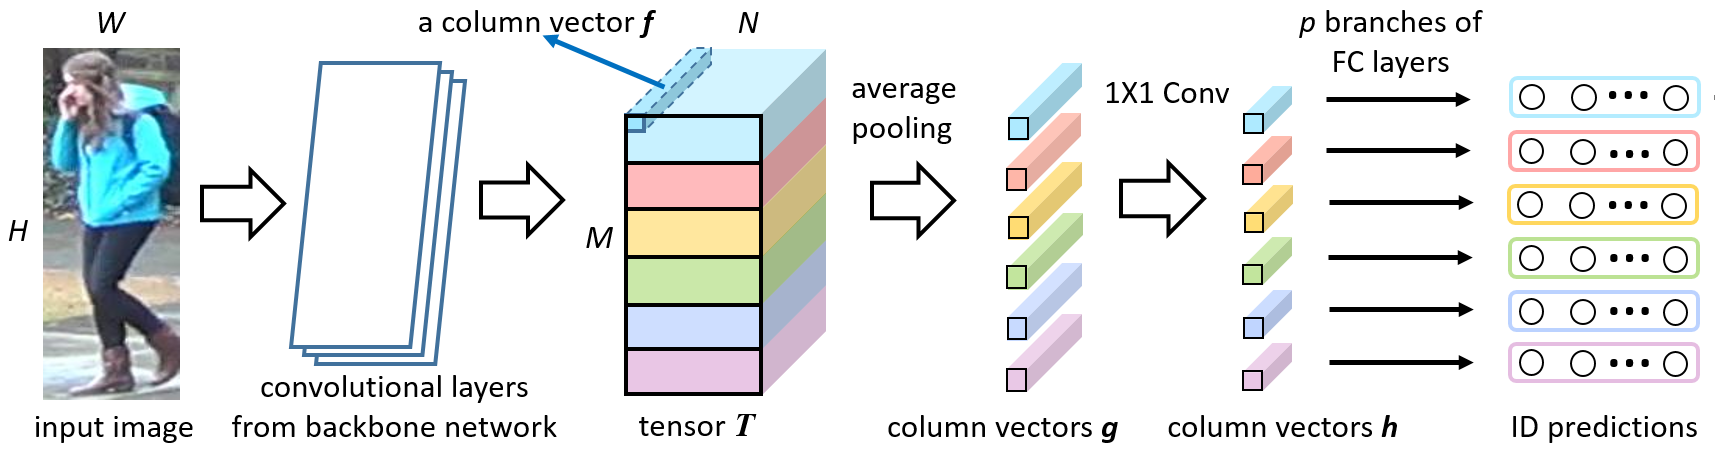
\includegraphics[width=1\textwidth]{structure}
\caption{Baseline架构图}
\label{fig:baseline}
\end{figure}

将ResNet50模型输出的特征图张量在竖直方向上分成$p=6$个水平条(Horizontal Stripes),每个通道保持独立。每个水平条通过一个尺寸与水平条尺寸相同全局池化层,使得原本为矩形的水平条变为一个$1\times1$的像素点,再将其与同一水平条其他通道的像素点拼接起来得到一个$2048\times1\times1$的向量。因为每个水平条会得到一个特征向量,所以经过全局池化层之后可得到$p$个向量,每一个向量都能表示原图像在对应的水平条范围内的局部特征。此方法的优点是简单、高效、易实现,缺点是每个人各部位的分布不同,人物上所具备的关注点也千差万别,将特征图张量在竖直方向上均匀分割不能很好地体现人与人之间的这些差异。

得到$p$个2048维的特征向量之后,再使用核尺寸为$1\times1$的卷积层将每个2048维的向量降为256维,以减少之后分类任务的计算量。每一个局部特征向量后接一个$n$分类器以预测该图像的类别,其中$n$为训练集中label的个数。训练的损失函数(Loss Function)使用交叉熵损失(Cross Entropy Loss)。

在测试阶段,即特征提取阶段,将最后的$p$个$n$分类器去掉,直接将$p$个256维的向量拼接(concatenate)为向量$\boldsymbol{g}$或将$p$个2048维的向量拼接为向量$\boldsymbol{h}$作为原始行人图像的特征表示。

\subsection{经过修正的分块池化算法}

基于分块卷积的基线模型将特征图张量在竖直方向上均匀分成$p$个水平条,以获得行人各部位的特征。此方法有操作简单、运算量少、易于实现的优点,但获取的分块过于粗糙,若要进一步获取行人各部分更精确的视觉信息,有必要在基线模型的基础上进行改进,不再局限于一个规范的矩形,而是通过计算判断每一个像素点「应该属于」哪一个部分。根据Sun等人的工作\cite{sun2017beyond},本项目中采取的经过修正的分块池化(Refined Part Pooling,RPP)算法示意图如图\ref{fig:refined}所示。在特征图上的每一个像素点不再简单地被均匀划分到相应的部分,而是根据当前行人图片的特征,动态地预测该像素点属于哪一个部分。

\begin{figure}[!htb]
\centering
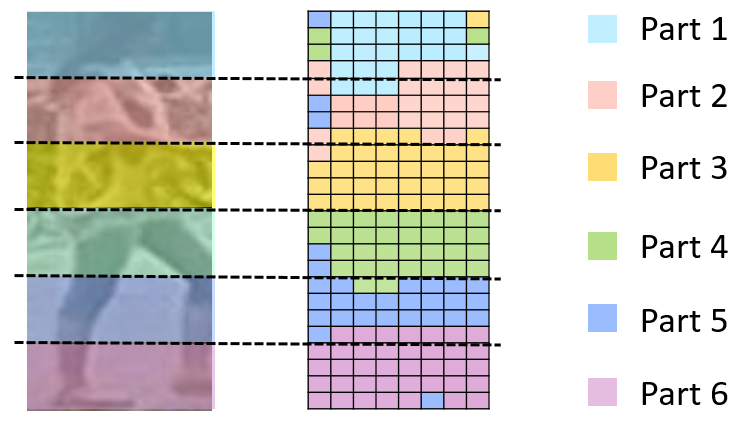
\includegraphics[width=6.67cm]{outliers1}
\caption{Refined Part Pooling示意图\cite{sun2017beyond}}
\label{fig:refined}
\end{figure}

经过修正的分块池化算法的目标为给定一个列向量(column vector,表示不同通道、相同位置的像素点),判断其属于哪一个部分。这就变成了一个分类问题。在这里使用一个线性神经网络层,来将所有的列向量分类。线性神经网络层有权重$W$和偏置$b$组成,为了简化表示,这里省略偏置$b$。对于一个列向量$f$,其属于第$i$个部分的概率$P(p_i\,\vert\,f)$为:
\begin{equation}
P(p_i\,\vert\,f)=\mathop{\rm softmax}\left(W_i^{\rm T}f\right)=\frac{\exp\left(W_i^{\rm T}f\right)}{\sum_j^p\exp\left(W_j^{\rm T}f\right)}
\end{equation}
其中$p_i$表示特征图的第$i$部分。

在基线模型中,列向量$f$只绝对的属于某一个部分。在求得$P(p_i\,\vert\,f)$后,则可将原始的列向量$f$按照概率分布分配到各部分。对于第$i$个部分$p_i$,其计算方式为:
\begin{equation}
p_i=\frac{1}{H\times W}\sum_{j=1}^{H\times W}P(p_i\,\vert\,f_j)\times f_j
\end{equation}
其中$H$、$W$分别代表特征图的高和宽。

如此一来即可得到与基线模型(PCB)前半部分等价的输出。再经过与PCB后半部分相同的$1\times1$卷积层和分类器,便完成了经过修正的分块池化算法 (RPP)算法的训练模型。完整的PCB+RPP架构图如图\ref{fig:structure2}所示。

\begin{figure}[!htb]
\centering
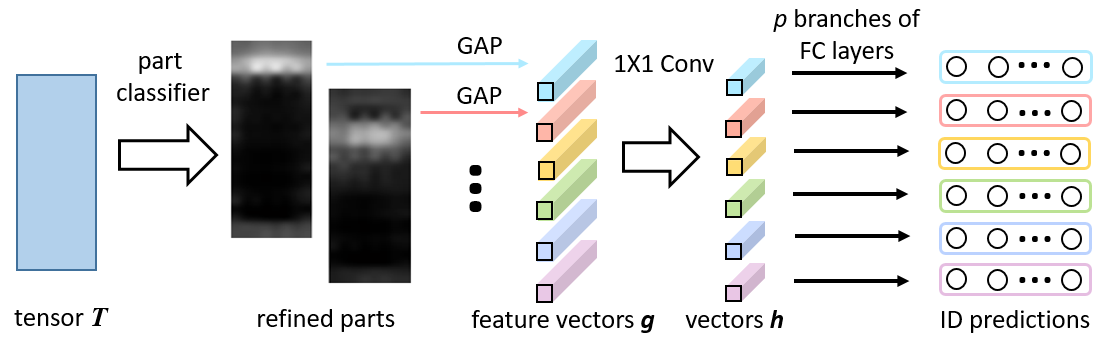
\includegraphics[width=1\textwidth]{structure2}
\caption{PCB+RPP架构图}
\label{fig:structure2}
\end{figure}

\section{监控摄像头部署方案的评价指标}

监控摄像头的部署方案包括摄像头的数量以及部署位置。摄像头的部署位置会影响监控场景的完整性、监控画面的光线质量以及监控目标的呈现角度。而监控摄像头数量受成本预算的限制,不可能无限增加,因此在预算有限的约束下,如何设计监控摄像头的部署位置,使得监控效果最优,便成为一个值得研究的问题。在研究优化问题之前,需要定义监控摄像头部署方案的评价指标$\mathcal{E}$。

监控效果的优劣可以定义为在当前的监控方案下,跨摄像头追踪特定行人的能力。当前在多摄像头多行人追踪(Multi-Target Multi-Camera Tracking,MTMC Tracking)领域主流的评价指标有多目标跟踪准确度($\mathit{MOTA}$)\cite{ristani2016MTMC}和识别F~值($\mathit{IDF_1}$)\cite{ristani2016MTMC}。

\subsection{多目标跟踪准确度($\mathit{MOTA}$)}

多目标跟踪准确度(Multiple Object Tracking Accuracy,$\mathit{MOTA}$)是衡量多目标追踪效果的常见指标。对于一段视频,其画面帧的总数为$T$,那么该段视频的多目标追踪准确度($\mathit{MOTA}$)的定义为:
\begin{equation}
\label{eq:mota}
\mathit{MOTA}=1-\frac{\mathit{FP}+\mathit{FN}+\Phi}{T}
\end{equation}
其中$\mathit{FN}$是视频所有帧中将负样本预测为正的总数,$\mathit{FP}$是视频所有帧中将正样本预测为负的总数,$\Phi$是预测序列中标签跳变的次数。$\mathit{MOTA}$指标的值域为$(-\infty,1]$,越接近1代表跟踪的效果越好。

\subsection{识别F值($\mathit{IDF_1}$)}

相比与$\mathit{MOTA}$中更多地关注目标人群的召回率以及目标追踪的稳定性,识别F值(Identification F-Score,$\mathit{IDF_1}$)更关注多摄像头多行人追踪过程中,行人标签的准确率。对于一段总帧数为$T$的视频,其识别F值($\mathit{IDF_1}$)定义为:
\begin{equation}
\mathit{IDF_1}=\frac{2\times\mathit{IDTP}}{2\times\mathit{IDTP}+\mathit{IDFP}+\mathit{IDFN}}
\end{equation}
其中$\mathit{IDTP}$是视频所有帧中将人物标签预测准确的总和,$\mathit{IDFP}$是视频所有帧中将正样本的人物标签预测错误的总和,$\mathit{IDFN}$是视频所有帧中将负样本的人物标签预测错误的总和。

\subsection{评价指标与当前的数据库结合}

结合本项目的实际情况,以及第一次预拍摄收集到的数据集的特点,将原始的17个摄像头中的第1个作为行人重识别算法的图库图片来源,其余16个摄像头按照物理位置和拍摄画面分为$G=5$组,每组摄像头个数为2至4个不等,定义$N=16$为待分配的摄像头总数,第$i$组的摄像头个数为$C_i$,同一组内摄像头大致拍摄到同一个物理位置,代表人物监控追踪场景中重点关注的位置。第$i$组的第$j$个摄像头定义为$c_{i,j}$,摄像头$c_{i,j}$的画面帧集合为$\mathcal{I}_{c_{i,j}}$。假设在预算有限的前提下,每个位置(每个分组)只能选择1个摄像头,如何从组内选择合适的摄像头,使得监控效果最佳,便是需要解决的问题。该优化问题可以用数学语言形式化表示为:
\begin{equation}
\max \left\{\mathcal{E}\left[\mathcal{F}\left(\sum_{i=1}^G \mathcal{I}_{c_{i,j}}\right)\right]\,\middle\vert\, 1\leq i \leq G, 1\leq j \leq C_i\right\}
\end{equation}
其中$\mathcal{I}_{c_x}+\mathcal{I}_{c_y}$表示摄像头$c_x$的视频数据与摄像头$c_y$的视频数据在时序上依次拼接。$\mathcal{E}[\mathcal{F}(\mathcal{I})]$表示对视频数据$\mathcal{I}$做多目标跟踪准确度($\mathit{MOTA}$)或识别F值($\mathit{IDF_1}$)评估。

\section{强化学习模型}

强化学习(Reinforcement Learning)是近年来十分流行的人工智能算法,相比于监督学习(Supervised Learning),强化学习不需要整个环境(Environment)所有情况的监督信息,只需要环境在某种特定的情况下给出相应的反馈(Reward)。在很多现实问题当中,优化空间的状态个数可能是个非常大的数字,且很证明是否收集到足够多样本,可以用来近似代表位置环境状态的分布。同时,在围棋问题\cite{silver2016mastering}中,各状态空间很难用监督的方法给每个状态评估价值,而强化学习只需要环境在每次动作(Action)之后给出相应的反馈,即可逐渐向更优的方向前进。强化学习也不属于无监督学习(Unsupervised Learning),无监督学习对于出现在测试集却不在训练集的样本没有处理能力,只能错误地分到已有的类中,而强化学习可以应对没有遇到的情况。

强化学习模型中的一般形式是一个智能体(Agent)在一个客观的环境(Environment)中,每一个时刻处于一个状态(State),当前状态存在一个短期价值和长期价值,短期价值可以是采取某种动作(Action)之后得到的反馈(Reward),长期价值(Value)则表示当前状态到最终状态能够得到的所有反馈总和的最大值。智能体根据当前状态的短期或长期价值和某种策略(Policy)采取某种动作,可立刻得到得到环境的反馈(Reward),并据此按照状态转移规则转移到下一个状态。在本项目中,根据要解决的具体问题,将上述概念相应定义如下:

当前的状态的集合$S=\left\{\boldsymbol{s}\,\middle\vert\,\boldsymbol{s}\in\mathbb{R}^{N}, s_i\in\{0, 1\}\right\}$,其中$s_i=1$表示选择了第$i$个摄像头。智能体可以采取的动作集合为$A=\left\{\boldsymbol{a}\,\middle\vert\,\boldsymbol{a}\in\mathbb{R}^N,\boldsymbol{a}_i \in \{0,1\}\right\}$,按照策略 $P$ 来选择动作, 1 表示选择该摄像头,0表示不选该摄像头。在本项目中,进行了动作之后, 状态是确定的,不存在一个动作可能导致几个不同的后续状态的情况,即状态转移概率 $\pi\left(\boldsymbol{s}^t\,\middle\vert\,\boldsymbol{s}^{t-1}, \boldsymbol{a}\right)\equiv1$。执行动作之后得到的反馈$r=\mathcal{E}\left[\mathcal{F}\left(\mathcal{I}^{(t+1)}\right)\right]-\mathcal{E}\left[\mathcal{F}\left(\mathcal{I}^{(t)}\right)\right]$,其中$\mathcal{I}^{(t)}$表示$t$时刻的视频数据,由$t$时刻的状态$\boldsymbol{s}^{(t)}$决定。当前状态 $S$ 的长期价值$V:\,S\mapsto\mathbb{R}^N$,是一个可学习的变量,代表智能体对于当前环境的认识程度。智能体应对当前状态的策略$P:\,V\mapsto A$,是长期价值 $V$ 到动作 $A$ 的映射,可以简单地用贪心的策略,即选择概率最高的 5 个摄像头。也可以用 Policy Network ,即深度神经网络来实现。在本项目中采用简单的贪心策略实现。

按照以上定义,智能体的一个动作就是选择一个合法的摄像头部署方案。对于一个动作,它的反馈就是下一个状态的性能指标$\mathcal{E}$($\mathit{MOTA}$ 或 $\mathit{IDF_1}$)减去当前状态的性能指标。在反馈已知的前提下,适合用 Q-Learning\cite{watkins1989learning} 算法。在Q-Learning算法中,智能体关于当前状态的长期价值表示为一个价值矩阵$Q$。Q-Learning算法首先随机初始化各个状态的长期价值,让智能体在环境中随机游走,每走一步会得到一个反馈,根据反馈更新当前状态的长期价值,直到收敛。智能体从而可学习出一个对于该环境的认知。本项目中使用Q-Learning算法求当前状态的长期价值如算法\ref{alg:qlearning}所示,其中最关键的算法在于如何更新长期价值$Q$,更新的公式中包含两个参数学习率$\alpha$和远见性$\gamma$,学习率$\alpha$表示$Q$的更新速度,远见性$\gamma$的取值范围为$(0, 1)$,表示智能体对于当前反馈与长远价值的重视程度,$\gamma$越大,代表越重视长远价值。

\begin{algorithm}[!htb]
    \caption{Q-Learning 算法求当前状态的长期价值}
    \label{alg:qlearning}
    \begin{algorithmic}[1]
        \Require 状态集合$S$、动作集合$A$、生命周期数$N$、学习率$\alpha$、远见性$\gamma$
        \Ensure 长期价值矩阵$Q$
        \Function {QLearning}{$S, A, N, \alpha, \gamma$}
            \State 随机初始化长期价值矩阵$Q$
            \For{$i=0\to N$}
                \State $\boldsymbol{s}^{(0)}\gets\boldsymbol{s}^\star$,$\boldsymbol{s}^\star$为从状态集合$S$中随机初始化的智能体的状态
                \State $t\gets1$
                \Repeat
                    \State $\boldsymbol{a}^{(t)}\gets \boldsymbol{a}^\star$,$\boldsymbol{a}^\star$为从动作集合$A$中随机选取的动作
                    \State $\boldsymbol{s}^{(t+1)}\gets \pi\left(\boldsymbol{s}^{(t)}, \boldsymbol{a}^{(t)}\right)$
                    \State $r^{(t)}\gets R\left(\boldsymbol{s}^{(t+1)},\boldsymbol{s}^{(t)}\right)$
                    \State $Q\left(\boldsymbol{s}^{(t)},\boldsymbol{a}^{(t)}\right)\gets(1-\alpha)\times Q\left(\boldsymbol{s}^{(t)},\boldsymbol{a}^{(t)}\right)+\alpha\times\left[r^{(t)}+\gamma\times\max_{\boldsymbol{a}'}Q\left(\boldsymbol{s}^{(t+1)}, \boldsymbol{a}'\right)\right]$
                    \State $\boldsymbol{s}^{(t)}\gets\boldsymbol{s}^{(t+1)}$
                    \State $t\gets  t+1$
                \Until{$\boldsymbol{s}^{(t)}=\boldsymbol{s}^{(0)}$}
            \EndFor
            \State\Return $Q$
        \EndFunction
    \end{algorithmic}
\end{algorithm}

\section{面向CPU集群的分布式深度学习训练框架}

计算机集群是一种计算机组织的物理形态,它是由一组彼此连接的计算机组成的,这些计算机一般协同完成同一项计算任务。在同一集群中每台计算机的内部结构可以不同,特别地,若集群中每台计算机主要的算力提供者是CPU,那么称该集群为CPU集群。分布式计算是计算的一种工作方式,它将一个计算任务划分成多个子任务,每一个子任务与其它子任务相对独立,可以在时间上并行计算,以缩短计算时间。CPU集群提供了一组在物理上相对独立的计算机,所以可以很自然地考虑将分布式计算中的各个子任务部署到CPU集群中,充分利用CPU集群的计算资源。

深度神经网络模型的训练过程一般可分为前馈计算(Forward)、误差反向传播(Loss Backpropagation)和参数更新。其中前向计算和反向传播的计算量很大,而且可以针对不同的训练集进行同步计算,因此深度神经网络模型的训练过程在结构上很适合进行分布式训练。在本项目中,集群的数量$n=5$,每个节点属于天河二号的GPU分区,具备高性能的CPU和GPU计算资源,节点之间通过千兆网络连接,避免各节点的通信速度成为分布式计算的性能瓶颈。

分布式训练架构如图\ref{fig:dist}所示,将训练数据通过随机采样的方式平均分成$n$份,分别输入集群中的各计算机。每一台计算机内存中包含一个独立的深度神经网络模型,进行该份训练数据的前馈计算和反向传播计算,得到该批次训练数据在当前模型下的各参数梯度。参数服务器的计算任务是收集集群中各计算机回传的梯度,更新模型参数,并将新参数分发给各计算机,各计算机得到新参数后进行下一批次训练数据的计算。更新模型参数的方法为:
\begin{eqnarray}
\Delta W=\frac{1}{n}\sum_{i = 1}^{n}\Delta W_i \\
W=W-\eta\Delta W
\end{eqnarray}
其中$\eta$是参数的学习率。

\begin{figure}[!htb]
\centering
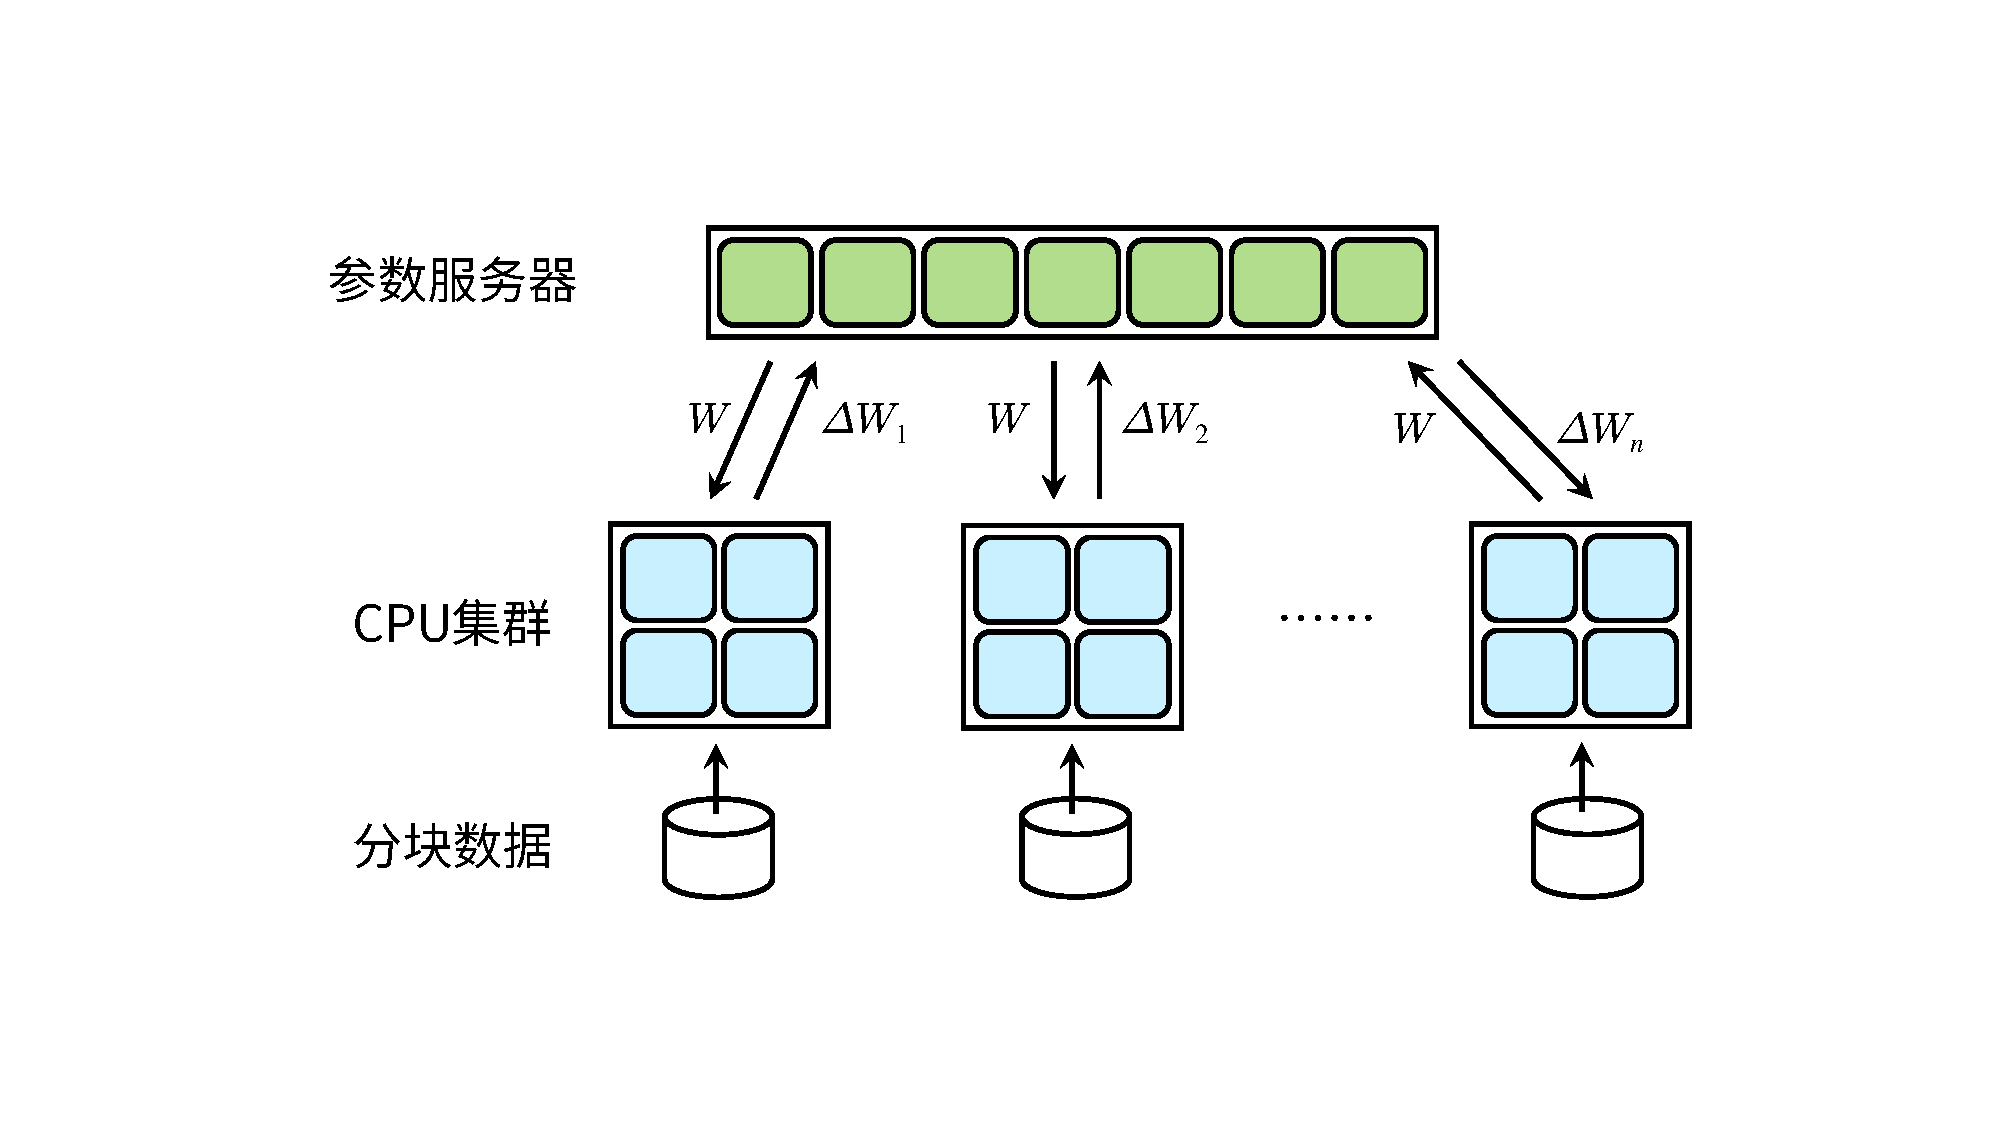
\includegraphics[width=0.7\textwidth]{dist}
\caption{分布式神经网络训练架构图}
\label{fig:dist}
\end{figure}